
\usepackage{fancyhdr}
\usepackage{lastpage}
\usepackage[utf8]{inputenc}

% Minted for syntax highliting
\usepackage{minted}
\usemintedstyle{tango}

% Headers/footers styling
\pagestyle{fancy}
\fancyhf{}
\renewcommand{\headrulewidth}{0pt}

% Footer
\lfoot{ID1019}
\cfoot{KTH}
\rfoot{\thepage \hspace{1pt} / \pageref{LastPage}}

%\newcommand{\defaultpagestyle}{\thispagestyle{plain}}
\newcommand{\defaultpagestyle}{\thispagestyle{fancy}}


\title[ID1019 Ray Tracer]{A Ray Tracer}
 
 
\author{Johan Montelius}
\institute{KTH}
\date{\semester}

\begin{document}

\begin{frame}
\titlepage
\end{frame}

\begin{frame}{A programming example}

To show how to work with some Erlang programming constructs and to
discuss representation and modeling, we will implement a small ray tracer. 

\pause \vspace{20pt}

\begin{figure}
 \includegraphics[scale=0.1]{world.jpg}
\end{figure}

\end{frame}

\begin{frame}{Architecture}

modules that we will implement

\begin{itemize}
 \item {\bf vector:} vector arithmetic
 \item {\bf objects:} representation and intersection of rays an objects
 \item {\bf camera:} the camera position, direction and characteristics
 \item {\bf tracer:} responsible for the tracing of rays 
 \item {\bf ppm:} how to generate a .ppm file
\end{itemize}

\pause and possibly some more

\end{frame}

\begin{frame}{ray tracing}

The basic idea of ray tracing: 

\begin{figure}
\begin{tikzpicture}[
        scale=0.4,
        axis/.style={very thick, ->, >=stealth'},
        important line/.style={thick},
        dashed line/.style={dashed, thin},
        pile/.style={thick, ->, >=stealth', shorten <=2pt, shorten >=2pt},
        every node/.style={color=black}
    ]
    % axis
    \draw[axis] (-1,0)  -- (19,0) node(xline)[right] {$x$};
    \draw[axis] (0,-1) -- (0,10) node(yline)[above] {$y$};

    \draw (16,8) circle (2);
    \pause

    \filldraw[red] (9,-4) rectangle (10,-3) node(eye)[below right]{Eye};
    \pause 
    \draw[red, thick] (6,1) node(canvas)[left] {Canvas} -- (13,1);
    \pause
    \draw[red, dashed] (5,-6) rectangle (14,2) node(camera)[right]{Camera};
    \pause
    \draw [pile] (9.5,-3) -- (14.5,6.5) node(hit)[left]{Intersection}; 
\end{tikzpicture}
\end{figure}
\end{frame}

\begin{frame}{vector arithmetic}

We first need a module to handle vector arithmetic:

\vspace{20pt}\pause

\begin{itemize}
  \pause \item Do we need to handle vectors of arbitrary dimensions?
  \pause \item How do we represent vectors?
  \pause \item What basic operations should we implement?
\end{itemize}
\end{frame}

\begin{frame}[fragile]{vector arithmetic}
\begin{columns}
 \begin{column}{0.5\linewidth}
  \begin{itemize}
   \item $a\vec{x}$ : scalar multiplication
   \item $\vec{x} - \vec{y}$ : subtraction
   \item $\vec{x} + \vec{y}$ : addition

  \end{itemize}
  \end{column}
  \pause

  \begin{column}{0.5\linewidth}
  \begin{itemize}
   \item $\|\vec{x}\|$ : norm, or length, of a vector
   \item $\vec{x} \cdot \vec{y}$ : scalar product (dot product)
   \item $|\vec{x}|$ : normalized vector $|\vec{x}| = \vec{x}/\|\vec{x}\|$
  \end{itemize}
  \end{column}
 \end{columns}

\vspace{40pt}

\pause {\em The notation for a normalized vector differ, sometimes it
  is written as $\hat{x}$}

\end{frame}


\begin{frame}[fragile]{vector arithmetic}

\begin{verbatim}
-module(vector).
-export([smul/2, add/2, sub/2, norm/1, normalize/1, dot/2]).
\end{verbatim}

\begin{columns}
 \begin{column}{0.5\linewidth}
  \begin{verbatim}
smul({X1,X2,X3}, S) ->  
    {X1*S, X2*S, X3*S}.
  \end{verbatim}
\pause
  \begin{verbatim}
sub({X1,X2,X3},{Y1,Y2,Y3}) -> 
    {X1-Y1,X2-Y2,X3-Y3}.
  \end{verbatim}
\pause
  \begin{verbatim}
add({X1,X2,X3},{Y1,Y2,Y3}) -> 
    {X1+Y1,X2+Y2,X3+Y3}.
  \end{verbatim}
  \end{column}

  \pause

  \begin{column}{0.5\linewidth}
  \begin{verbatim}
norm({X1,X2,X3}) ->
   math:sqrt(X1*X1+X2*X2+X3*X3).
  \end{verbatim}
\pause
  \begin{verbatim}
dot({X1,X2,X3},{Y1,Y2,Y3}) ->
    X1*Y1 + X2*Y2 + X3*Y3.
  \end{verbatim}
\pause
  \begin{verbatim}
normalize(X) ->
    N = norm(X),  smul(X, 1/N).
  \end{verbatim}
  \end{column}
 \end{columns}

\end{frame}

\begin{frame}[fragile]{objects}

The module {\tt objects} should define how to represent objects and functions that can be applied to objects.

\pause
\begin{itemize}
  \item rays: origin and direction
  \item spheres: origin, radius, ...
 \end{itemize}

\end{frame}

\begin{frame}[fragile]{rays}

  A ray is defined by an origin and a direction. The origin is a
  vector (a place in the space) and the direction is a {\em unit
    vector}.

\pause 

\begin{columns}[T]
 \begin{column}{0.3\linewidth}
  \begin{figure}
   \begin{tikzpicture}[
        scale=0.3,
        axis/.style={very thick, ->, >=stealth'},
        important line/.style={thick},
        dashed line/.style={dashed, thin},
        pile/.style={thick, ->, >=stealth',  shorten >=2pt},
        every node/.style={color=black}
    ]
    % axis
    \draw[axis] (-1,0)  -- (10,0) node(xline)[right] {$x$};
    \draw[axis] (0,-1) -- (0,10) node(yline)[above] {$y$};
    \draw[fill] (3,4) node(o)[below left]{$\vec{o}$} circle (4pt);
    \draw[pile] (3,4)  -- (4,6) node()[right]{$\vec{l}$};
    \draw[dashed] (3,4) -- (7,12);
   \end{tikzpicture}
  \end{figure}  
  \end{column}

\pause

\begin{column}{0.7\linewidth}

\begin{verbatim}
#ray{origin, direction}
\end{verbatim}


\begin{verbatim}
ray(Org, Dir) -> #ray{origin=Org, direction=Dir}
\end{verbatim}

  \end{column}
 \end{columns}
\end{frame}

\begin{frame}[fragile]{tuples and records}

 \begin{itemize}
  \item a vector: {\tt \{2, 3, 1\}}
  \item a ray:  {\tt \#ray\{origin=\{3,4,0\}, direction=\{0.447, 0.894, 0\}\}}
 \end{itemize}

\pause\vspace{20pt}

\verb+-record(ray, {origin, direction})+

\pause \vspace{10pt}
\verb+#ray{origin={3, 2, 4}, direction={0.447, 0.894, 0}}+

\pause \vspace{10pt}
\verb+#ray{origin=Org} = Ray+

\pause \vspace{10pt}
\verb+Org = Ray#ray.origin+

\end{frame}


\begin{frame}[fragile]{spheres}

A sphere is defined by:
\vspace{20pt}\pause

\begin{columns}[T]
 \begin{column}{0.3\linewidth}
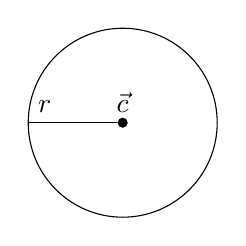
\begin{tikzpicture}[
        scale=0.4,
        important line/.style={thick},
        dashed line/.style={dashed, thin},
        pile/.style={thick, ->, >=stealth', shorten >=2pt},
        every node/.style={color=black}
    ]
    \draw (3,6) node(r)[above right]{$r$} -- (6,6);
    \draw[fill] (6,6) node()[above]{$\vec{c}$} circle (4pt);
    \draw (6,6) circle (3);
\end{tikzpicture}

 \end{column}
\pause
 \begin{column}{0.7\linewidth}
\begin{verbatim}
-record(sphere, {radius, center}).

sphere(Rd, Cntr) ->
   #sphere{radius=Rd, center=Cntr}.

\end{verbatim}

 \end{column}
\end{columns}

\vspace{20pt}\pause
{\em more properties will be added later}
\end{frame}


\begin{frame}{intersection}


\begin{columns}
 \begin{column}{0.4\linewidth}
\begin{figure}
\begin{tikzpicture}[
        scale=0.4,
        important line/.style={thick},
        dashed line/.style={dashed, thin},
        pile/.style={thick, ->, >=stealth', shorten >=2pt},
        every node/.style={color=black}
    ]
    \draw[fill] (6,6) node()[above]{$\vec{c}$} circle (4pt);
    \draw (6,6) circle (3);

    \draw<2-|handout:1>[fill] (4,-3) node()[below left]{$\vec{o}$} circle (4pt);

    \draw<2-|handout:1> [dashed](4,-3) -- (11,11); 

    \draw<3-|handout:1> [thick,pile](4,-3) -- (5,-1) node(l)[right]{$\vec{l}$};  

    \draw<4-|handout:1>  (7,3) node(i1)[below right]{$\vec{i_1}$};
    \draw<4-|handout:1>  (9,6) node(i1)[right]{$\vec{i_2}$};

    \draw<5-|handout:1> [thick, pile] (4,-3) -- (6,6);
    \draw<5-|handout:1>  (3.5,2) node(k)[]{$\vec{k}$};

    \draw<7-|handout:1> [dashed] (6,6) -- (8,5);

    \draw<7-|handout:1>[dashed] (6,6) -- (10,4);  %% (4, -2)

    \draw<7-|handout:1>[dashed] (4,-3) -- (6,-4);   %% (2,-1)

    \draw<7-|handout:1>[dashed] (6,-4) -- (10,4) node()[midway, right] {$a$};

    \draw<8-|handout:1> (7,6) node()[]{h};

    \draw<10-|handout:1> [dashed] (6,6) -- (7,3);
    \draw<10-|handout:1> (6.2,4) node()[]{r};

    \draw<11-|handout:1> (8,4) node()[]{t};
\end{tikzpicture}
\end{figure}
 \end{column}
\pause 
\begin{column}{0.6\linewidth}
  \pause
  \begin{itemize}
   \uncover<6-|handout:1>{\item $\vec{k} =  \vec{c} - \vec{o}$}
   \uncover<7-|handout:1>{\item $a = \vec{l}\cdot\vec{k}$}
   \uncover<9-|handout:1>{\item $\|k\|^2 = a^2 + h^2$}
   \uncover<12-|handout:1>{\item ${r}^2 =  h^2 + t^2$}
   \uncover<13-|handout:1>{\item $ t^2 = {a}^2  - \|k\|^2   + {r}^2 $}
   \uncover<14-|handout:1>{\item $\vec{i} = \vec{o} + d \vec{l}$}
   \uncover<15-|handout:1>{\item $ d_i = a\pm t$}
   \uncover<16-|handout:1>{\item if $d_i < 0$ then $\vec{i_i}$ is {\em behind} the origin $\vec{o}$}
  \end{itemize}
 \end{column}
\end{columns} 
\end{frame}


\begin{frame}[fragile]{objects:intersect/2}

\begin{columns}
 \begin{column}{0.6\linewidth}
\begin{verbatim}
intersect(#sphere{radius=R, center=C}, #ray{origin=O, direction=L}) ->

    K = vector:sub(C,O),
    A = vector:dot(L, K),
    A2 = math:pow(A, 2),
    K2 = math:pow(vector:norm(K),2),
    R2 = math:pow(R,2),
    T2 = A2 - K2 + R2,
    closest(T2, A).
\end{verbatim}
 \end{column}
\pause
 \begin{column}{0.4\linewidth}

  $$\vec{k} =  \vec{c} - \vec{o}$$
  $$a = \vec{l}\cdot\vec{k}$$
  $${t}^2 = {a}^2 - \|k\|^2 + {r}^2 $$
  $$d = a\pm t$$
 \end{column}
\end{columns}
\end{frame}

\begin{frame}[fragile]{objects:closest/2}

\begin{columns}
 \begin{column}[T]{0.6\linewidth}
\begin{verbatim}
closest(T2, A) ->
    if  T2 < 0 ->   no;
        true -> 
            T = math:sqrt(T2),
            D1 = A - T,  D2 = A + T,
            if 
                (D1 > 0.0) and (D2 > 0.0) ->  {ok, min(D1,D2)};
                (D1 > 0.0) -> {ok, D1};
                (D2 > 0.0) -> {ok, D2} ;
                true -> no
            end
    end.
\end{verbatim}
 \end{column}
\pause
 \begin{column}[T]{0.4\linewidth}
  if $t^2$ < $0$, there is no intersection. 

  if $d_i < 0$, $\vec{i_i}$ is behind the origin $\vec{o}$ of the ray
 \end{column}
\end{columns}


\end{frame}

\begin{frame}{ok, what else?}

\begin{figure}
\begin{tikzpicture}[
        scale=0.4,
        axis/.style={very thick, ->, >=stealth'},
        important line/.style={thick},
        dashed line/.style={dashed, thin},
        pile/.style={thick, ->, >=stealth', shorten <=2pt, shorten >=2pt},
        every node/.style={color=black}
    ]
    % axis
    \draw[axis] (-1,0)  -- (19,0) node(xline)[right] {$x$};
    \draw[axis] (0,-1) -- (0,10) node(yline)[above] {$y$};

    \draw (16,8) circle (2);
    \pause
    \filldraw[red] (9,-4) rectangle (10,-3) node(eye)[below right]{Eye};
    \pause 
    \draw[red, thick] (6,1) node(canvas)[left] {Canvas} -- (13,1);
    \pause
    \draw[red, dashed] (5,-6) rectangle (14,2) node(camera)[right]{Camera};
    \pause
    \draw [pile] (9.5,-3) -- (14.5,6.5) node(hit)[left]{Intersection}; 
\end{tikzpicture}
\end{figure}

\end{frame}

\begin{frame}[fragile]{the camera}


\begin{columns}
 \begin{column}{0.5\linewidth}

\begin{figure}
 \includegraphics[scale=0.4]{olympusom1.jpg}
\end{figure}

 \end{column}

 \begin{column}{0.5\linewidth}
What properties do we have?
  \begin{itemize}
 \pause \item position : in space
 \pause \item direction : a unit vector 
 \pause \item size of picture : width and height
 \pause \item focal length : distance to canvas
 \pause \item resolution: pixles per distance
  \end{itemize}
 \end{column}

\end{columns}

\end{frame}

\begin{frame}[fragile]{a simple camera}

\begin{verbatim}
-module(camera).

-export([normal/2, size/1, ray/3).

-record(camera, {pos,    % camera position
                 corner, % picture position
                 right,  % one pixle right
                 down,   % one pixle down
                 size,   % {width, height}
                }).
\end{verbatim}

\end{frame}


\begin{frame}[fragile]{a normal lens pointing forward}

\begin{verbatim}
normal(Pos,  Size) ->
    {Width, Height} = Size,
    Direction = {0,0,1}, 

    Distance = trunc(math:sqrt(math:pow(Width,2) + math:pow(Height, 2))),
    Center = vector:add(Pos, vector:smul(Direction, Distance)),

    Corner = vector:add(Center, {-trunc(Width/2),trunc(Height/2),0}), 
    Right = {1, 0, 0},
    Down =  {0,-1, 0},

    #camera{pos=Pos, corner = Corner, 
            right=Right, down=Down, size= Size}.

\end{verbatim}

\end{frame}


\begin{frame}[fragile]{rays}

Given a camera we want to find the rays from the camera ``origin'' to
the \{x,y\} position of the canvas.

\pause

\begin{verbatim}
ray(X, Y, Camera) ->
    Origin = Camera#camera.pos,
    Xpos = vector:smul(Camera#camera.right, X),
    Ypos = vector:smul(Camera#camera.down, Y),
    XYpos = vector:add(Xpos, Ypos),
    Pos = vector:add(Camera#camera.corner, XYpos),
    Dir = vector:normalize(vector:sub(Pos, Origin)),
    objects:ray(Origin, Dir).
\end{verbatim}

\end{frame}


\begin{frame}{we have everything}

\begin{figure}
\begin{tikzpicture}[
        scale=0.4,
        axis/.style={very thick, ->, >=stealth'},
        important line/.style={thick},
        dashed line/.style={dashed, thin},
        pile/.style={thick, ->, >=stealth', shorten <=2pt, shorten >=2pt},
        every node/.style={color=black}
    ]
    % axis
    \draw[axis] (-1,0)  -- (19,0) node(xline)[right] {$x$};
    \draw[axis] (0,-1) -- (0,10) node(yline)[above] {$y$};

    \draw (16,8) circle (2);
    \pause
    \filldraw[red] (9,-4) rectangle (10,-3) node(eye)[below right]{Eye};
    \pause 
    \draw[red, thick] (6,1) node(canvas)[left] {Canvas} -- (13,1);
    \pause
    \draw[red, dashed] (5,-6) rectangle (14,2) node(camera)[right]{Camera};
    \pause
    \draw [pile] (9.5,-3) -- (14.5,6.5) node(hit)[left]{Intersection}; 
\end{tikzpicture}
\end{figure}

\end{frame}


\begin{frame}[fragile]{the tracer}

\begin{verbatim}
-module(tracer).

-export([tracer/2]).

tracer(Camera, Objects) ->
    {W, H} = camera:size(Camera),
    Xs = lists:seq(1, W),
    Ys = lists:seq(1, H),
    [[trace(X, Y, Camera, Objects) || X <- Xs] || Y <- Ys].

trace(X, Y, Camera, Objects) ->
    Ray = camera:ray(X, Y, Camera),
    trace(Ray, Objects).
\end{verbatim}

\end{frame}

\begin{frame}[fragile]{tracing a ray}

\begin{verbatim}
trace(Ray, Objects) ->
    case intersect(Ray, Objects) of
        {inf, _} ->
            ?Black;
        {_, _} -> 
            ?White
    end.
\end{verbatim}

\end{frame}

\begin{frame}[fragile]{the last piece}

\begin{verbatim}
intersect(Ray, Objs) ->
   lists:foldl(fun(Obj, Sofar) -> 
                       {Dist, _} = Sofar,
                       case objects:intersect(Obj, Ray) of
                           {ok, D} when D < Dist ->
                               {D, Obj};
                           _ ->
                               Sofar
                       end
               end,
               {inf, no},
               Objs).
\end{verbatim}

\end{frame}

\begin{frame}[fragile]{time to test}
\begin{verbatim}
-module(test).

-compile(export_all).

snap()->
    Camera = camera:normal({0,0,-800}, {600,400}),

    Obj1 = objects:sphere( 140, {   0,    0,    -100}),
    Obj2 = objects:sphere(  50, { 200,    0, -200}),

    Rows = tracer:tracer(Camera, [Obj1, Obj2]),

    ppm:write("test0.ppm", Rows).
\end{verbatim}
\end{frame}

\begin{frame}{test0.ppm}

\begin{figure}
\includegraphics[scale=0.3]{test0.png};
\end{figure}

\end{frame}


\begin{frame}[fragile]{colors}

\pause Let's add some colors to the spheres.

\begin{verbatim}
-define(Color, {1.0,0.4,0.4}).

-record(sphere, {radius=2, center, color=?Color}).

-export([sphere/2, sphere/3, intersect/2, color/1]).
\end{verbatim}
\pause
\begin{verbatim}
sphere(Radius, Center, Opt) ->
    Color = case lists:keyfind(color, 1, Opt) of
                {color, C} ->
                    C;
                false ->
                    ?Color
            end,
    #sphere{radius=Radius, center=Center, color=Color}.
\end{verbatim}

\pause
\begin{verbatim}
color(#sphere{color=Color}) ->  Color.
\end{verbatim}

\end{frame}

\begin{frame}[fragile]{small change to the tracer}

\pause
\begin{verbatim}
ray(Ray, Objects) ->
    case intersect(Ray, Objects) of
        {inf, _} ->
            ?Black
        {_, Obj} -> 
            objects:color(Obj).
    end.
\end{verbatim}
\end{frame}


\begin{frame}[fragile]{time to test}
\begin{verbatim}

snap() ->
    Camera = camera:normal({0,0,-800}, {600,400}),

    Obj1 = objects:sphere(140, {0,0,-100}, [{color, {200,100,0}}]),
    Obj2 = objects:sphere(50, {200,0,-200}, [{color, {0,200,50}}]),
    Obj3 = objects:sphere(50, {-80,0,-400}, [{color, {0,200,50}}]),

    Rows = tracer:tracer(Camera, [Obj1, Obj2, Obj3]),

    ppm:write("test1.ppm", Rows).
\end{verbatim}
\end{frame}

\begin{frame}{test1.ppm}

\begin{figure}
\includegraphics[scale=0.3]{test1.png};
\end{figure}

\end{frame}



\begin{frame}{adding lights}

\pause We want to add some lights to the world.

\pause 
\vspace{10pt}Lights have a position and a color

\pause 
\vspace{10pt}The color of an intersection point is determined by the color of the object combined with the colors from the lights. 

\pause 
\vspace{10pt}Things are getting interesting.

\end{frame}

\begin{frame}[fragile]{two more modules}

\begin{itemize}
\item {\bf lights:} handles everything that has to do with lights and colors.
\item {\bf world:} describes objects, lights, background etc
\end{itemize}

\pause 
\vspace{20pt} the representation of colors is a RGB tuple of floats 0..1.0 i.e. \verb+{1.0, 0.5, 0.2}+
\end{frame}



\begin{frame}[fragile]{normal vector}


\begin{columns}
 \begin{column}{0.4\linewidth}
\begin{figure}
\begin{tikzpicture}[
        scale=0.4,
        important line/.style={thick},
        dashed line/.style={dashed, thin},
        pile/.style={thick, ->, >=stealth', shorten >=2pt},
        every node/.style={color=black}
    ]

    \draw (6,6) node(c)[above]{$\vec{c}$} circle (3);
    \draw [dashed] (4,-3) node(o)[below left]{$\vec{o}$} -- (11,11);  

    \draw [dashed] (c) -- (7.1,3.2) node(i)[]{};

    \draw (i) node[right = 0.4cm]{$\vec{i}$};

    \draw [thick, pile] (i) -- (8.19, -0.42) node(n)[right]{$\vec{n}$};
\end{tikzpicture}
\end{figure}
 \end{column}
\pause
 \begin{column}{0.6\linewidth}
$\vec{n}$ is the normal unit vector, i.e. perpendicular to the sphere, at the point of intersection.
  $$\vec{n} = |\vec{i} - \vec{c}|$$
\pause 

Will come in handy when we calculate reflection and illumination.

 \end{column}
\end{columns}

\end{frame}

\begin{frame}[fragile]{the world}

 \pause A more convenient way to handle lack of  globally accessible data structures.

\begin{verbatim}
-module(world).
-export([world/2, world/3, background/1, ambient/1, lights/1, objects/1]).

-define(Background, {0,0,0}).
-define(Depth, 2).
-define(Ambient, {0.3,0.3,0.3}).

-record(world, { objects=[], 
                 lights=[], 
                 background=?Background, 
                 depth=?Depth, 
                 ambient=?Ambient
               }).
\end{verbatim}

\end{frame}

\begin{frame}[fragile]{calculating the color}

Find all visible lights from the point of intersection; combine the lights give the normal vector and illuminate the surface.
\pause

In the tracer: \pause

\begin{verbatim}
{D, Obj} -> 
    O = objects:origin(Ray),
    L = objects:direction(Ray),

    I = vector:add(O, vector:smul(L, (D-?Delta))),

    Normal = objects:normal(I, Obj),

    Visible = visible(I, world:lights(World), Objs),

    Illumination = lights:combine(I, Normal,  Visible),

    lights:illuminate(Obj, Illumination, World)
\end{verbatim}
\end{frame}


\begin{frame}[fragile]{visible lights}

\begin{verbatim}
visible(Point, Lights, Objs) ->
    lists:filter(fun(Light) -> 
                    clear(Point, lights:origin(Light), Objs)  
                 end, 
                 Lights).
\end{verbatim}

\end{frame}


\begin{frame}[fragile]{lights}

\begin{verbatim}
-module(lights).

-export([light/2, origin/1, illuminate/3, combine/3,  rgb255/1]).

-record(light, {origin, color={1.0,1.0,1.0}}).

light(Origin, Color) ->
    #light{origin=Origin, color=Color}.

origin(#light{origin=Origin}) ->
    Origin.
\end{verbatim}

\end{frame}


\begin{frame}[fragile]{lights}

\pause 
combine two light sources

\pause 
\begin{verbatim}
add({R1,G1,B1}, {R2,G2,B2}) ->
    {(1 - ((1-R1)*(1-R2))), (1 - ((1-G1)*(1-G2))), (1 - ((1-B1)*(1-B2)))}.
\end{verbatim}

\pause 
\vspace{20pt}
illuminate a colored surface with a colored light

\begin{verbatim}
ill({R1,G1,B1}, {R2,G2,B2}) ->
   {R1*R2, G1*G2, B1*B2}.
\end{verbatim}

\end{frame}

\begin{frame}[fragile]{the angle of lights}

\pause 
a light contributes proportional to the cosine of the angle 
\pause 

\begin{verbatim}
contribute(Point, Normal, Source, {R,G,B}) ->
    Direction = vector:normalize(vector:sub(Source, Point)),
    Cos = (vector:dot(Direction, Normal)),
    {R*Cos, G*Cos, B*Cos}.
\end{verbatim}

\pause 
\vspace{20pt} we combine lights by adding their contribution

\begin{verbatim}
combine(Point, Normal, Lights) ->
    lists:foldl(fun(#light{origin=Src, color=Clr}, Contr) -> 
                  add(contribute(Point, Normal, Src, Clr), Contr)
                end,  
                {0,0,0},
                Lights).
\end{verbatim}

\end{frame}

\begin{frame}{test2:ppm}

\begin{figure}
\includegraphics[scale=0.2]{test2.png};
\end{figure}

\end{frame}



\begin{frame}{the fun part}

The color of an intersection point depends on:

\begin{itemize}
 \pause \item color of the object
 \pause \item combination of light sources 
 \pause \item reflection from other objects
\end{itemize}

\end{frame}

\begin{frame}[fragile]{the depth}

\begin{verbatim}
trace(X, Y, Camera, World) ->
    Ray = camera:ray(X, Y, Camera),
    Depth = world:depth(World),
    trace(Ray, Depth, World).
\end{verbatim}

\pause 
\begin{verbatim}
trace(_Ray, 0, World) ->
    world:background(World);
trace(Ray, Depth, World) ->
      :
\end{verbatim}

\end{frame}


\begin{frame}[fragile]{the recursive call}

\pause 
\begin{verbatim}
     Ref = objects:ray(I, reflection(L, Normal)),

     Reflection = trace(Ref, Depth-1, World),

     lights:illuminate(Obj, Reflection, Illumination, World)
\end{verbatim}

\pause
\begin{verbatim}
reflection(L, N) ->
    vector:sub(L,vector:smul(N,2*vector:dot(L,N))).
\end{verbatim}

\end{frame}

\begin{frame}{test3:ppm}

\begin{figure}
\includegraphics[scale=0.2]{test3.png};
\end{figure}

\end{frame}


\begin{frame}{what more}

This was only scratching the surface of ray tracing.

\end{frame}

\begin{frame}{from an architecture point of view}

\begin{itemize}
 \pause \item divide program into areas of responsibility
 \pause \item think about abstractions
 \pause \item modules are similar to class definitions
 \pause \item a static type system would have helped us (records are only halfway)
\end{itemize}

\end{frame}

\end{document}
